\section{DataBase design}
In this section is presented the structure of the database which supports
the activities of the AllSpark organization.
In order to provide a more clear picture of the structure the database is
divided in different sections. 

Each one of this supports a different section of the organization, briefly
they are:
\begin{description}
\item[Administration: ] Provide support for the employees, projects and
customer organization.
\item[Project: ] Here are stored all the information of the projects on
which the organization is working.
\item[Resources: ] This part provides support for hosting the resources of
the enterprise, such as documentation, project details.
\end{description}

\subsection{Administrative section}
This section of the information system provides support for the
administrative part of AllSpark organization.
In particular it handles the employees administration, with their
specialization and roles. The activity classes permits to track a log of
each worker activity and to plan future event as meetings or deadlines.

Moreover it manages the inventory of the organization, which is mainly
composed by software and hardware (servers, network infrastructures). It
contains the references to the suppliers list, in order to retrieve
informations who supplied each item used in the organization.

In this part of the database is stored even the customer and their
relative contracts details. The image in \ref{3img:classadmin} shows the
details of this database in the form of a class diagram.

\begin{figure}[H]
\centering
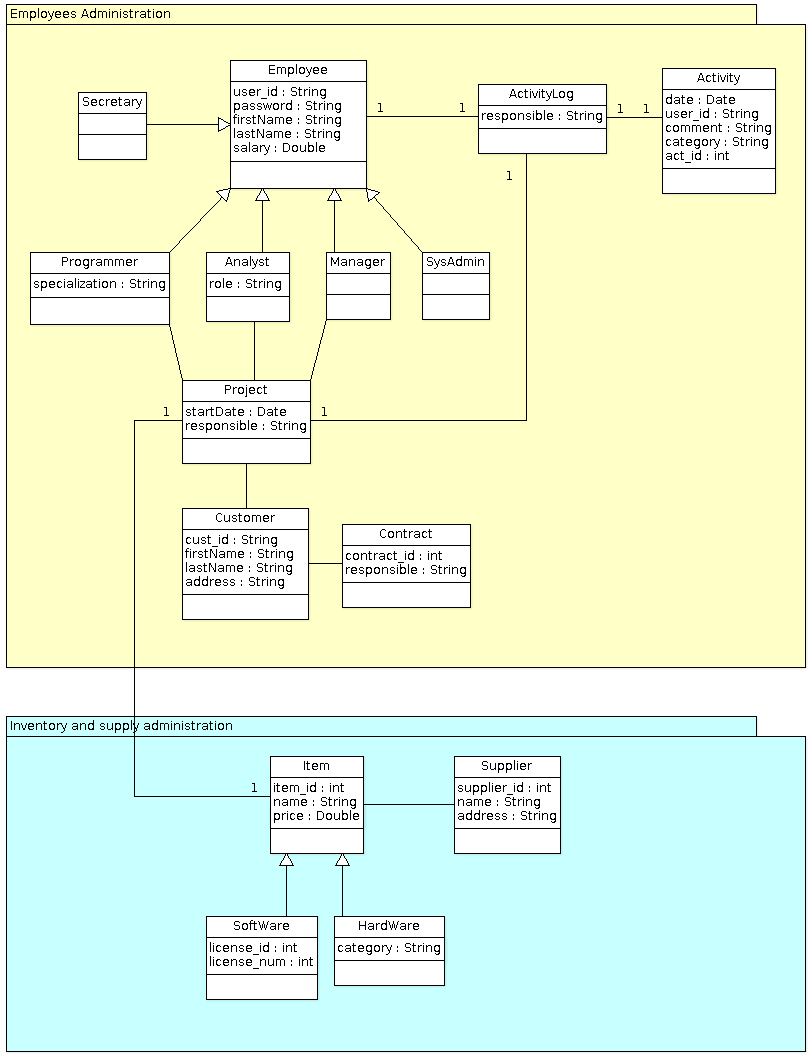
\includegraphics[scale=0.50]{assign3/argo/imgs/administrative.png}
\caption{Class diagram describing the administration database}
\label{3img:classadmin}
\end{figure}

\subsection{Project Section}
The branch of the database which manages the handling of the data related
to the projects is depicted in figure \ref{3img:classprj}.
One of the relevant thing is the managing of the budget specific for each
project, In fact every resource used for the project, which often is an
hardware resource or an intervention of technical assistance (internal or
external), is accounted on the project budget.

Other parts of the database maintain the informations about the various
teams which cooperates in the project, specifying their roles and members.
For a human resource point of view, the actors involved in a project
lifecycle are usually a manager and a variable number of developers and
analysts. 

The case of a research project falls into the general definition of a
common project, effectively, from a data point of view, there are no
relevant differences between the two kind of projects.

\begin{figure}[H]
\centering
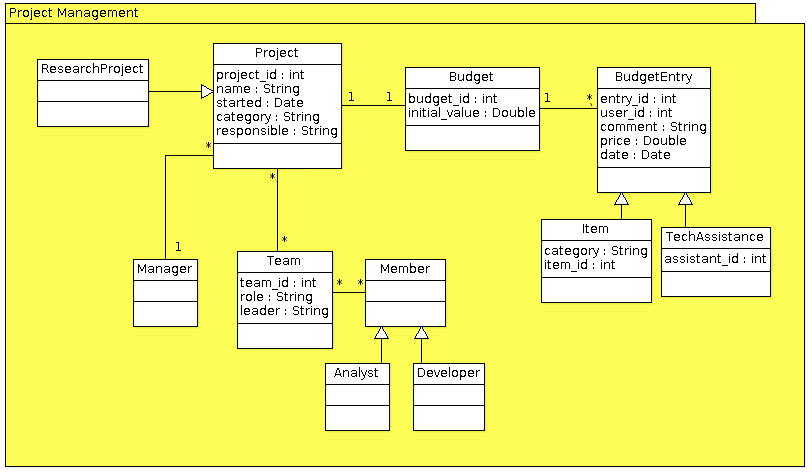
\includegraphics[scale=0.50]{assign3/argo/imgs/project.png}
\caption{Class diagram describing the project branch of the database}
\label{3img:classprj}
\end{figure}

\subsection{Documents and resources section}
This section of the database holds the data used for the management of the
document needed by the organization. These resources are mainly
documentation for projects and systems and documents for requirement
analysis and other project management tasks.

The system provides support for tracking all the modification done over a
resource, storing the user and the changelog of his intervention. This is
not to be intended as a revision management system, which is not in the
scope of AllSparks information systems, but it provides a log all the
activities performed.

Another feature is the access control, organized in the form of groups of
users which have different permission level on the resource.
Picture \ref{3img:classres} depicts this structure.

\begin{figure}[H]
\centering
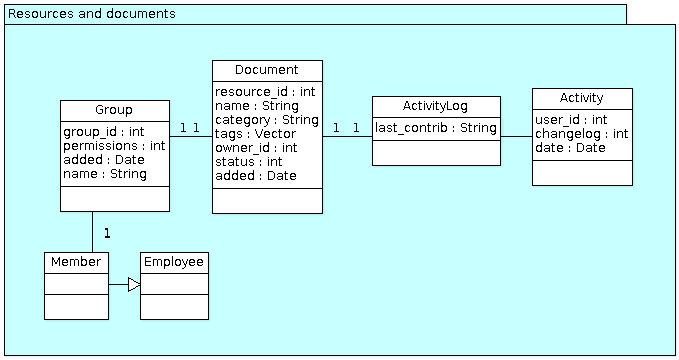
\includegraphics[scale=0.60]{assign3/argo/imgs/resources.png}
\caption{Class diagram describing the resource part of the database}
\label{3img:classres}
\end{figure}

\section{Courses section}
The organization of the formative courses is managed by a specific branch
of the database, and its structure is described by the class diagram in
figure \ref{3img:classcou}.
The information system permits to hold informations about the course
material used and about the lecturers for each course.

Another important feature is the association of the course with the
certification which grants. 
The database contains informations about the exam of the course, its
details and the dates in which it takes place.

The people who takes the course are considered as en extension  of
Customer, with some additional information about the hours of class
attended and the exam results.

\begin{figure}[H]
\centering
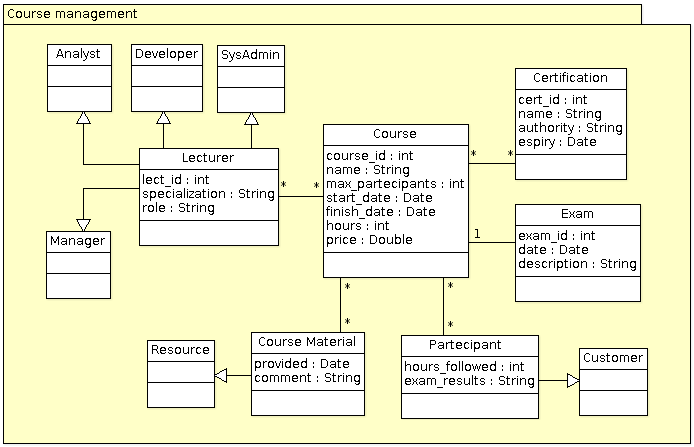
\includegraphics[scale=0.60]{assign3/argo/imgs/courses.png}
\caption{Class diagram describing the courses part of the database}
\label{3img:classcou}
\end{figure}

